\section{Vitis: Setting up the Software Side}

Vivado is used for the \gls{pl}-side of Zynq, and Vitis for the \gls{ps}-side. To setup properly:

\begin{enumerate}
    \item Create a folder inside c:\, or somewhere with a short pathname called workspace. If any files exceed the Windows limit of 256, the platform will not build.
    \item Open Vitis. Select Open Workspace, and open the workspace you just created.
    \item Select File -> New Component -> Platform.
    \item Give it a name (default is fine), ensure it will live inside workspace.
    \item Select next. Select Hardware Design and browse for the .xsa file inside the temp folder.
    \item Select next. Use Operating System standalong and the default processor. 
    \item Select Generate Boot Artifacts
    
    \begin{center}
        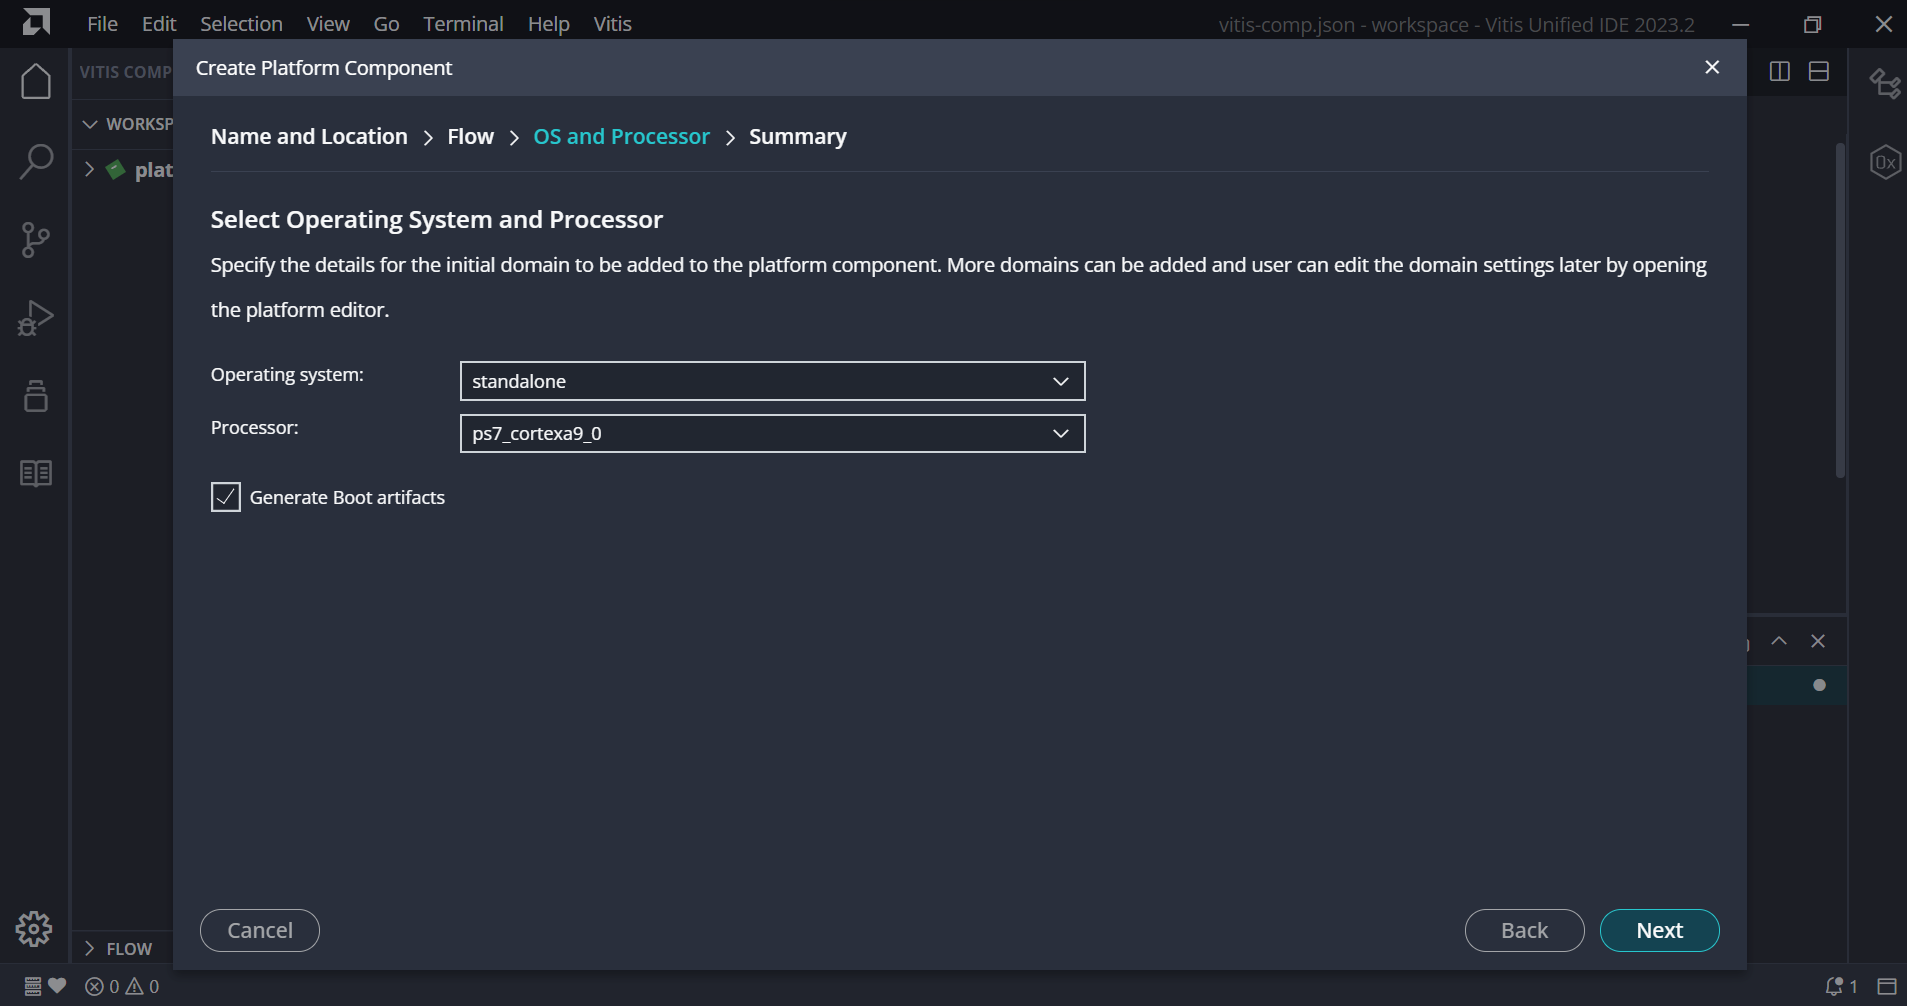
\includegraphics[width=0.9\textwidth]{aa_latex/Figures/Blink_LED/Vitis/vitis.png}
    \end{center}

    \item Select Next and Finish.
    \item Vitis should build the platform.
    
     \begin{center}
        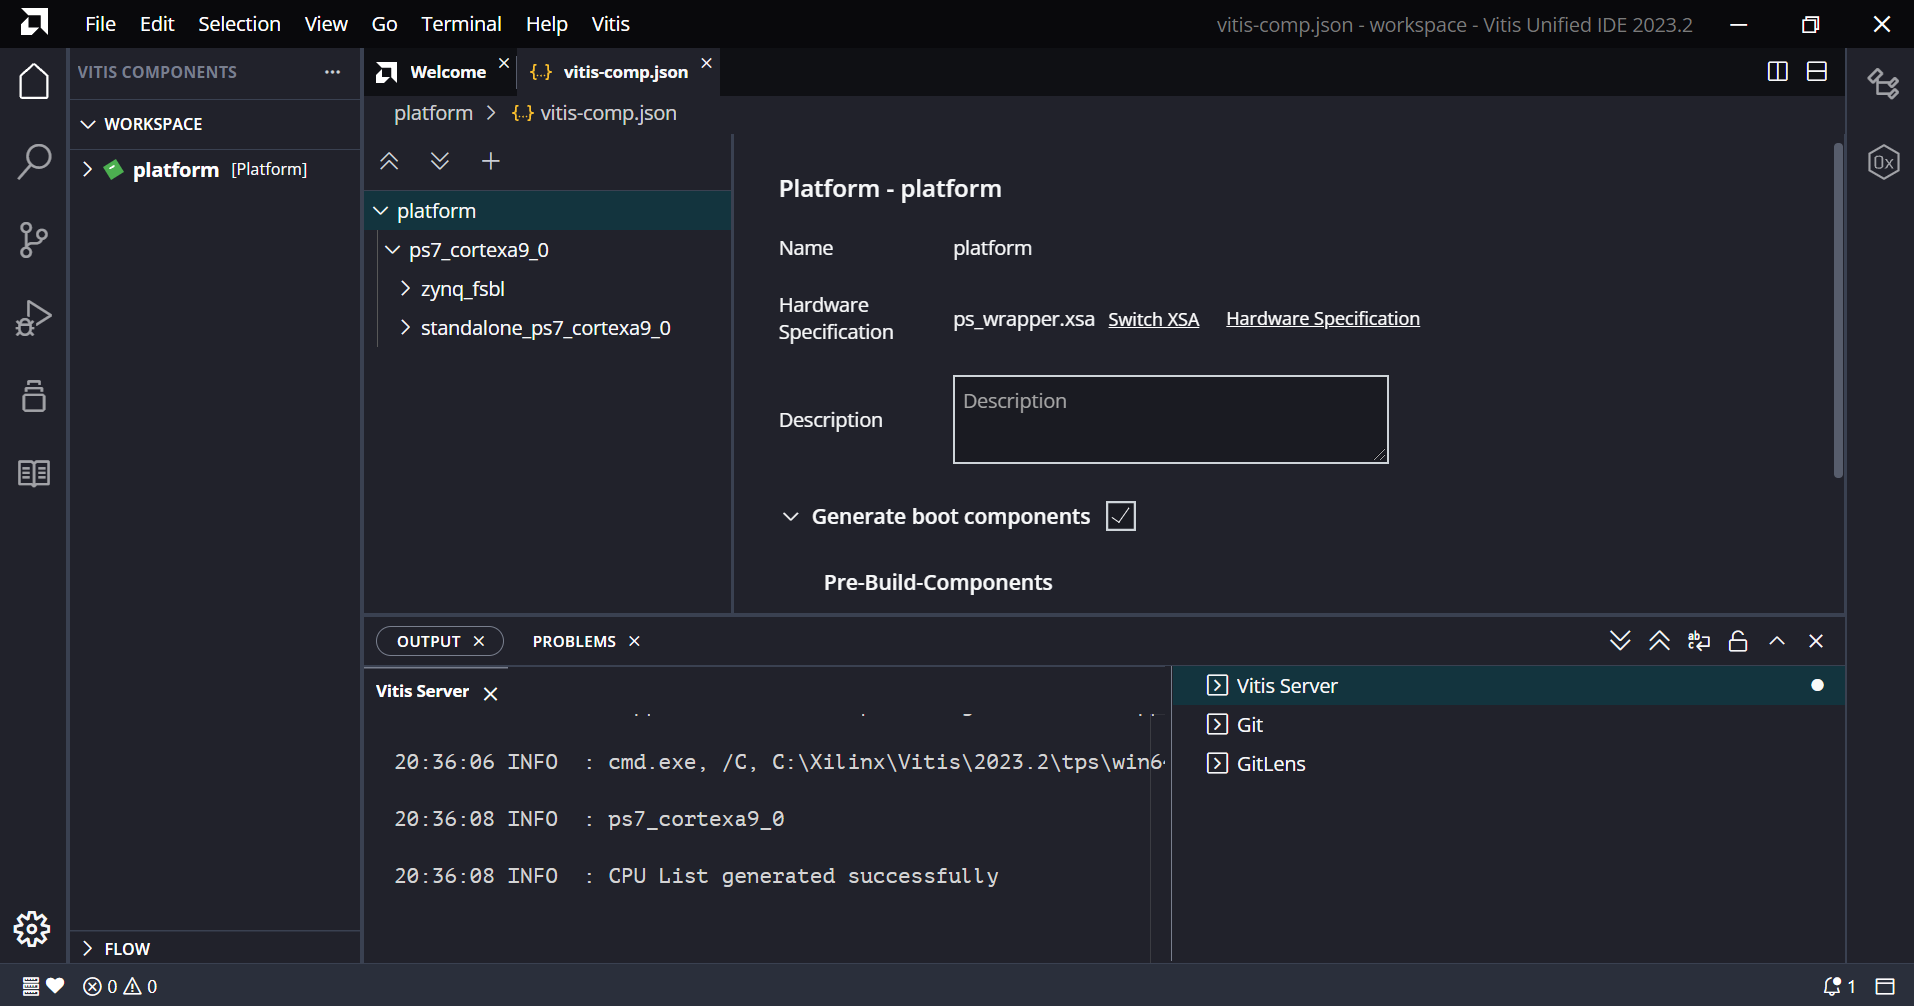
\includegraphics[width=0.9\textwidth]{aa_latex/Figures/Blink_LED/Vitis/platform.png}
    \end{center}
\end{enumerate}